\documentclass[11pt,a4paper]{book}

% ---------------- Balíčky ----------------
\usepackage[T1]{fontenc}
\usepackage[utf8]{inputenc}
\usepackage[czech]{babel}
\usepackage{lmodern}
\usepackage{graphicx}
\usepackage{geometry}
\usepackage{setspace}
\usepackage{hyperref}
\usepackage{longtable}
\usepackage{booktabs}
\usepackage{xcolor}
\usepackage{makeidx}
\usepackage{qrcode}
\usepackage[utf8]{inputenc}
\usepackage[most]{tcolorbox}

\makeindex

\geometry{margin=25mm}
\setstretch{1.2}

\definecolor{orang}{RGB}{255,155,0}

\makeatletter
\renewcommand\Huge{\@setfontsize\Huge{40pt}{48pt}}
\renewcommand\huge{\@setfontsize\huge{30pt}{36pt}}
\renewcommand\LARGE{\@setfontsize\LARGE{24pt}{30pt}}
\renewcommand\Large{\@setfontsize\Large{18pt}{22pt}}
\renewcommand\large{\@setfontsize\large{14pt}{18pt}}
\makeatother

\newtcolorbox[auto counter,number within=section]{caja}[1][]{
  enhanced jigsaw,colback=white,colframe=orang,coltitle=orang,
  fonttitle=\bfseries\sffamily\large,
  sharp corners,
  detach title,
  leftrule=22mm,
  underlay unbroken and first={\node[below,text=black,anchor=east]
  at ([xshift=-22.5pt]interior.base west) {\Huge  \textbf{!}};},
  breakable,pad at break=1mm,
  #1,
  code={\ifdefempty{\tcbtitletext}{}{\tcbset{before upper={\tcbtitle\par\medskip}}}},
}

% ---------------- Metadata ----------------
\title{\Huge \textbf{In-Time Server}\\[1em]
\LARGE Manuál v1.6}
\author{Paul Gingerbread}
\date{\today}

% ---------------- Dokument ----------------
\begin{document}

% ----- Titulní strana -----
\begin{titlepage}
    \centering
    \vspace*{2cm}
    
\includegraphics[width=0.45\textwidth]{img/intime_logo.pdf}\par
    \vspace{1cm}
    {\Huge \textbf{In-Time Server}\par}
    \vspace{0.5cm}
    {\Large Manuál v1.6\par}
    \vfill
    {\Large Paul Gingerbread\par}
    \vspace{1cm}
\end{titlepage}

% ----- Tiráž -----
\newpage
\thispagestyle{empty}
\vspace*{6cm}
\begin{center}
\qrcode{https://github.com/ontarioskaut/in_time} \\
\vspace{1cm}
\textbf{In-Time Server – Manuál v1.6}\\
Autor: Paul Gingerbread\\[1em]
Sazba a tisk: Systémové nakladatelství TimePress, Lidechko 2025\\
Náklad: 25 výtisků, první vydání\\
ISBN: 978-80-420-6900-0 \\


\end{center}
\newpage

\frontmatter
\tableofcontents

% ----- Úvod -----
\mainmatter
\chapter{Úvod}
\addcontentsline{toc}{chapter}{Úvod}

\textbf{In-Time Server Admin} je příkazová utilita pro správu a řízení běžícího časového serveru systému \emph{In-Time}. Tento server vyměřuje čas občanům Lidové časové federace a představuje klíčovou infrastrukturu, bez které by nemohly fungovat základní společenské procesy. Nástroj je určen výhradně pro členy \emph{časového výboru}, který nad systémem drží dohled, řídí jeho provoz a~nese za něj plnou odpovědnost. Inspirací je filmový svět \emph{In Time}, v němž čas není jen údaj na displeji, ale primární měna a zároveň délka života. Stejná logika zde platí i prakticky: jakákoliv změna v záznamech času se bezprostředně promítá do životů lidí.

Tento manuál poskytuje srozumitelný, ale detailní popis funkcí nástroje, jeho konfiguračních přepínačů a doporučených pracovních postupů. Cílem je, aby správce rozuměl nejen tomu, \emph{jak} příkaz spustit, ale hlavně \emph{co} jeho provedení znamená pro systém jako celek. Tam, kde je to potřeba, jsou uvedena bezpečnostní upozornění a kontrolní kroky (potvrzení, kontrolní otázky), které mají snížit riziko chyby obsluhy.

\medskip
\noindent\textbf{Na co je nástroj určen:}
\begin{itemize}
    \item \textbf{Monitoring stavu}~(\texttt{{-}{-}get\_active})~– rychlá kontrola, zda je systém aktivní a vykonává přidělování času.
    \item \textbf{Přehled časů uživatelů}~(\texttt{{-}{-}list\_user\_times})~– zobrazení tabulky se jmény, počátečním časem, uplynulou dobou a zbývajícím časem; včetně formátovaného výstupu a zvýraznění kritických stavů.
    \item \textbf{Evidence uživatelů a kategorií}~(\texttt{{-}{-}list\_users}, \texttt{--list\_categories})~– auditovatelný náhled do registru subjektů a jejich zařazení.
    \item \textbf{Auditní záznamy}~(\texttt{{-}{-}get\_logs})~– zpětná dohledatelnost zásahů a rozhodnutí.
    \item \textbf{Aplikace časových posunů}~(\texttt{{-}{-}apply\_user\_offset}, \texttt{--apply\_user\_cat})~– přesné, dávkové zásahy do zůstatků času jednotlivců nebo skupin.
    \item \textbf{Rozdělení alokace}~(\texttt{{-}{-}split\_allocated\_time})~– rovnoměrná distribuce dostupné alokace mezi všechny evidované subjekty.
    \item \textbf{Řízení provozních režimů}~(\texttt{{-}{-}set\_core\_mode}, \texttt{--authorize}, \texttt{{-}{-}set\_user})~– přístup do zvýšeně nebezpečných zón řízení, včetně vícestupňového potvrzení a autentizace.
    \item \textbf{Aktivace/deaktivace systému}~(\texttt{{-}{-}set\_active})~– řízené uvedení systému do aktivního stavu nebo jeho bezpečné zastavení.
\end{itemize}

\medskip
\noindent\textbf{Proč je opatrnost zásadní:} V prostředí In-Time systém neposkytuje pouze informaci; \emph{čas je hodnotou, která přímo určuje délku života}. Každé navýšení, snížení či reset zůstatku času proto představuje rozhodnutí s etickými i právními důsledky. Chybný příkaz, špatně zvolený parametr nebo neověřená dávková operace může znamenat reálné ztráty na životech. Z tohoto důvodu utilita záměrně vyžaduje:
\begin{itemize}
    \item víceúrovňové potvrzení u kritických operací,
    \item kontrolní otázky ověřující pozornost obsluhy,
    \item striktní oddělení režimů (\texttt{CORE\_MODE}, \texttt{AUTHORIZED\_MODE}) a identifikaci operátora,
    \item auditní záznamy všech zásahů pro následnou kontrolu a forenzní analýzu.
\end{itemize}

\medskip
\noindent\textbf{Rozsah a filosofie práce s nástrojem:} Manuál je psán pro zkušené správce, kteří rozumějí dopadům svých příkazů a přijímají odpovědnost za důsledky. Doporučené workflow vždy začíná diagnostikou (získání stavu, přehledu uživatelů a logů), pokračuje přípravou změn (simulace, výpočet offsetů, ověření cílové množiny) a končí \emph{reverzibilními} kroky všude tam, kde je to možné. \textbf{Než provedete zásah}, ověřte:
\begin{enumerate}
    \item že cíl a dopad změny jsou přesně vymezené,
    \item že parametry odpovídají záměru (uživatelé, kategorie, velikosti posunů),
    \item že existuje konzistentní auditní stopa a schválení časovým výborem,
    \item že běží správný režim a je nastavena identita obsluhy.
\end{enumerate}

\medskip
\noindent\textbf{Etické a provozní zásady:} Nástroj má být užíván výlučně ve prospěch stability a bezpečí federace. Jakékoliv testování provádějte odděleně od produkčního systému. V rámci produkce nikdy nespouštějte hromadné operace bez předchozího omezení rozsahu (např. na malý vzorek) a~bez dvojího ověření parametrů. V případě pochybností je správným postupem \emph{neprovádět} změnu a eskalovat ji časovému výboru.

\medskip
Následující kapitoly rozvádějí jednotlivé přepínače, návrhy pracovních postupů a doporučení pro bezpečný provoz. \textbf{Pamatujte}: v systému In-Time jsou čísla více než čísla; představují čas, a tím také život. Jednejte s maximální opatrností.

% ----- Uvedení do provozu -----
\mainmatter
\chapter{Uvedení do provozu}

\section*{Předmluva k provozu}
\noindent
\textbf{In-Time Server} je navržen jako spolehlivé, průmyslově robustní řešení pro nepřetržitý provoz. Kombinuje deterministické chování serverového Linuxu s pečlivě řízenými službami, které zajišťují konzistentní distribuci času napříč celým systémem. Díky jednoduché, ale auditovatelné správě a důslednému logování poskytuje správcům \emph{časového výboru} jistotu, že každý cyklus alokace i každá změna konfigurace je dohledatelná a reprodukovatelná. Architektura je od základu postavená na principech minimální závislosti, čitelného startu bez grafického splash screenu a~preferenci textových rozhraní --- aby bylo \emph{vždy} jasné, co se v systému děje.

\section{Zapojení}
\noindent
Před prvním spuštěním proveďte fyzické zapojení podle následujících kroků. Všechna připojení provádějte při vypnutém napájení serveru.

\begin{enumerate}
  \item \textbf{Napájení:} Připojte síťový kabel \textbf{230\,V AC} do zdroje v zadní části skříně serveru. Ujistěte se, že zásuvka odpovídá normě a je chráněna jističem a proudovým chráničem.
  \item \textbf{Síť/bezdrát:} Zasuňte \textbf{bezdrátový adaptér} (Wi\texttt{-}Fi) do \textbf{USB} portu v zadní části skříně. Preferujte porty přímo na základní desce pro vyšší stabilitu.
  \item \textbf{Audio výstup:} Vedení z reproduktorů (\textbf{3{,}5\,mm jack}) zapojte do \textbf{prostřední zelené zdířky} ve \textbf{spodnější řadě} audio konektorů na zadní straně počítače (standardní \emph{Line Out}).
  \item \textbf{Volitelně:} Připojte ethernetový kabel do RJ\texttt{-}45 (doporučeno pro management), monitor přes HDMI/DisplayPort a klávesnici do USB.
\end{enumerate}

Jakmile je vše zapojeno, systém je \textbf{připraven ke spuštění}. Doporučujeme vizuálně zkontrolovat všechny konektory a zajistit kabeláž proti náhodnému vytažení.

\medskip
\begin{figure}[h]
  \centering
  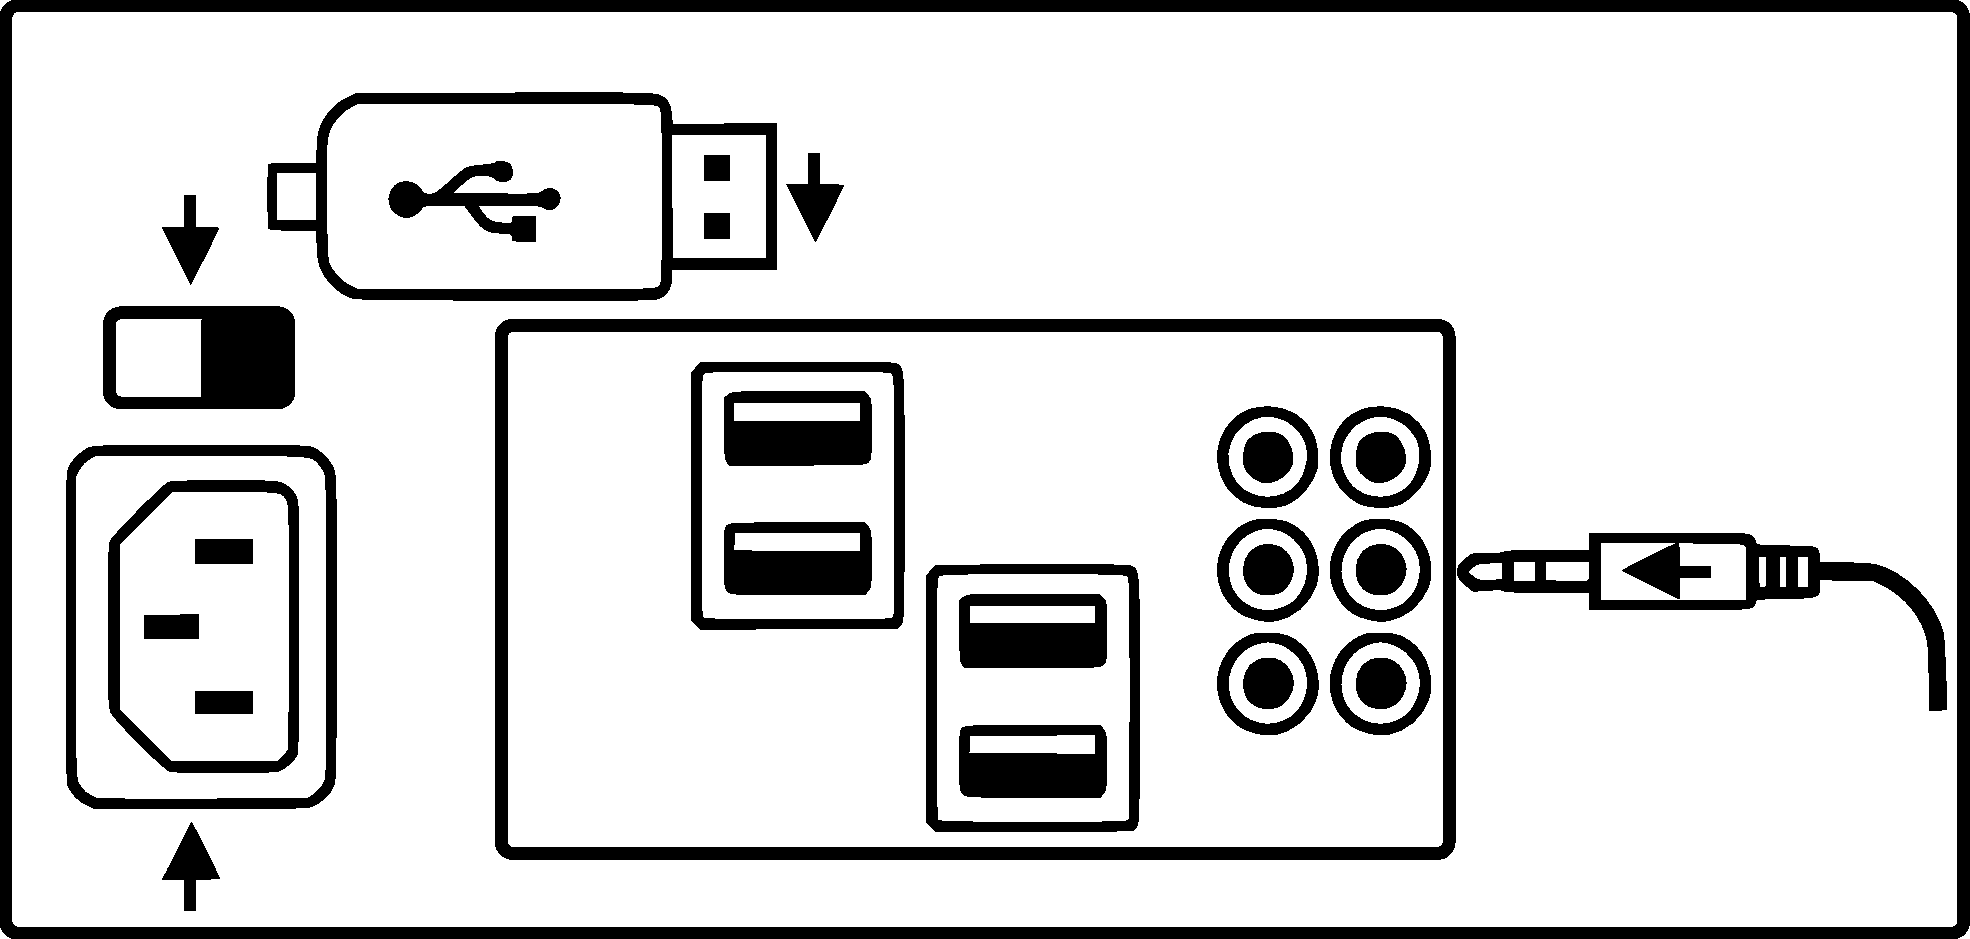
\includegraphics[width=0.9\textwidth]{img/pc_schema.pdf}\par
  \caption{Schéma zapojení systému In-Time (doplní se).}
\end{figure}

\section{Start}
\noindent
Server používá zavaděč \textbf{GRUB} a distribuci \textbf{Debian GNU/Linux}. Start je \textbf{bez grafického splash screenu}, takže na obrazovce uvidíte průběžné systémové hlášky.

\subsection{Fáze BIOS/UEFI (po zapnutí)}
Po zapnutí se objeví obrazovka \emph{POST} základní desky (logo výrobce, test paměti, detekce disků).
\begin{itemize}
  \item Typicky jsou dostupné klávesy \texttt{Del}/\texttt{F2} pro vstup do nastavení UEFI a \texttt{F11}/\texttt{F12} pro nabídku \emph{Boot Menu}.
  \item Zkontrolujte, že bootovací zařízení je nastaveno na disk se systémem (\emph{Linux}).
  \item Pokud se zde objeví varování o ventilátorech/napájení, vypněte a zkontrolujte hardware.
\end{itemize}

\subsection{Zavaděč GRUB}
Po \emph{POST} se zobrazí textová nabídka \textbf{GRUB}.
\begin{itemize}
  \item \textbf{Výchozí položka:} \texttt{Debian GNU/Linux}. Po krátkém odpočtu (obvykle 5\,s) se spustí automaticky.
  \item \textbf{Možnosti:} Může být k dispozici \texttt{Advanced options} (recovery jádra). Není\texttt{-}li nutné, ponechte výchozí.
  \item Typická hláška: \texttt{Loading Linux \dots\quad Loading initial ramdisk \dots}
\end{itemize}

\subsection{Načítání jádra a \emph{initramfs}}
V této fázi Linux jádro inicializuje zařízení a mountuje kořenový souborový systém.
\begin{itemize}
  \item Uvidíte strohé texty o detekci CPU, paměti, disků (NVMe/SATA), případně RAID/LVM.
  \item Při potížích s diskem se mohou objevit hlášky \texttt{EXT4-fs error}, \texttt{mount: special device not found} apod. V tom případě zkontrolujte kabeláž/UEFI nastavení.
\end{itemize}

\subsection{\texttt{systemd}: spouštění služeb}
Po předání řízení \texttt{systemd} začne start jednotlivých jednotek (\texttt{units}).
\begin{itemize}
  \item Vlevo se objevují stavové značky \texttt{[  OK  ]} / \texttt{[FAILED]} u služeb. Příklady, které běžně uvidíte:
  \begin{itemize}
    \item \texttt{[  OK  ] Reached target Basic System.}
    \item \texttt{[  OK  ] Started Network Manager.} \quad nebo \quad \texttt{Started ifupdown-pre.service}
    \item \texttt{[  OK  ] Started OpenSSH server daemon.}
    \item \texttt{[  OK  ] Reached target Multi-User System.}
    \item \texttt{[  OK  ] Started getty@tty1.service.}
  \end{itemize}
  \item \textbf{Bez splash screenu} uvidíte průběh detailně; jedná se o standardní chování a je žádoucí pro transparentní diagnostiku.
\end{itemize}

\subsection{Přihlašovací výzva (TTY1)}
Po startu systém přejde do textové přihlašovací obrazovky:
\begin{verbatim}
Debian GNU/Linux 13 intime_server tty1

intime_server login:
\end{verbatim}
\begin{enumerate}
  \item Zadejte \textbf{uživatelské jméno} a potvrďte \texttt{Enter}.
  \item Zadejte \textbf{heslo} (znaky se nezobrazují) a potvrďte \texttt{Enter}.
\end{enumerate}
Po přihlášení se zobrazí uvítací zpráva (\texttt{motd}) a shell prompt:
\begin{verbatim}
Welcome to Debian GNU/Linux 13 (trixie)!
user@intime_server:~$
\end{verbatim}

\paragraph{Poznámky a tipy:}
\begin{itemize}
  \item Pokud se \textbf{GRUB nezobrazí} a systém bootuje jiný OS, zkontrolujte pořadí boot zařízení v UEFI.
  \item \textbf{Dlouhé zpoždění} při \texttt{systemd} startu často souvisí s čekáním na síť. Ověřte kabeláž a~konfiguraci.
  \item V případě \texttt{[FAILED]} u služby pokračujte analýzou přes \texttt{journalctl} a opravte konfiguraci dříve, než systém uvedete do produkce.
\end{itemize}

\medskip
\noindent
\textbf{Důležité bezpečnostní upozornění:} Tento server přímo ovlivňuje životní čas občanů. Před přechodem do aktivního režimu vždy ověřte správnost konfigurace, časových zdrojů, připojení periferií a dostupnost síťových služeb. Každá chyba v této fázi může mít následky v produkčním provozu.

% ----- Příkazová řádka -----
\mainmatter
\chapter{Prostředí příkazové řádky}

\section{Co je \emph{shell} a jak do něj psát}
\noindent
\textbf{Shell} (též \emph{příkazová řádka}) je textové rozhraní, do kterého píšete příkazy. 
Po přihlášení do systému Debian uvidíte tzv. \emph{prompt} (výzvu), např.:
\begin{verbatim}
user@server:~$
\end{verbatim}
Blikající kurzor označuje místo, kam se bude vkládat text. Příkaz vytvoříte tak, že napíšete 
jeho název a případné argumenty/přepínače a potvrdíte klávesou \textbf{Enter}. Shell je 
\textbf{case-sensitive} (rozlišuje malá/velká písmena): `\texttt{Time\_Server}` není totéž jako `\texttt{time\_server}`.

\section{Základní editace a ovládání klávesnicí}
\noindent
Při psaní příkazů se hodí několik klávesových zkratek.

\begin{longtable}{@{}llp{8cm}@{}}
\toprule
\textbf{Klávesa} & \textbf{Akce} & \textbf{Poznámka} \\
\midrule
\texttt{$\uparrow$} / \texttt{$\downarrow$} & Historie & Prochází dříve zadané příkazy. \\
\texttt{$\leftarrow$} / \texttt{$\rightarrow$} & Pohyb kurzoru & Přesun o znak vlevo/vpravo. \\
\texttt{Home} / \texttt{End} & Začátek / Konec řádku & Rychlý přesun na okraj řádku. \\
\texttt{Tab} & Doplňování & Automatické doplnění názvů příkazů/souborů. \\
\bottomrule
\end{longtable}

\paragraph{Potvrzení příkazu.}
Příkaz se \textbf{nevykoná}, dokud nestisknete \textbf{Enter}. Pokud příkaz čeká na vstup 
(např. otázka \emph{„Proceed? [y/N]“}), odpovězte a opět potvrďte \textbf{Enter}.
\newpage
\section{Co je příkaz, argument a přepínač}
\noindent
\textbf{Příkaz} je program nebo vestavěná funkce shellu. Za názvem příkazu mohou následovat 
\textbf{argumenty} (hodnoty, cesty, čísla) a \textbf{přepínače} (volby), které mění chování příkazu.

\begin{verbatim}
time_server --list_user_times
^command   ^switch (dlouhý přepínač)
\end{verbatim}

\section{Tipy a triky}
Pokud nevíte, jaké argumenty u daného příkazu použít, většinou je dostupný přepínač \texttt{{-}{-}help}, který zobrazí úhlednou nápovědu, jak program používat.



% ----- Použití -----
\mainmatter
\chapter{Použití příkazu \texttt{time\_server}}
Utility se spouští příkazem:
\begin{verbatim}
$ time_server [PŘEPÍNAČE]
\end{verbatim}

Pouze jeden přepínač může být použit současně.

\section{Obecné přepínače}
\begin{longtable}{@{}llp{9cm}@{}}
\toprule
\textbf{Přepínač} & \textbf{Argumenty} & \textbf{Popis} \\
\midrule
\texttt{{-}-get\_active} & žádné & Zobrazí, zda je systém aktivní (True/False). \\
\texttt{{-}-list\_user\_times} & žádné & Vypíše tabulku uživatelů a jejich zbývajícího času. \\
\texttt{{-}-list\_users} & žádné & Podrobný seznam uživatelů v systému. \\
\texttt{{-}-list\_categories} & žádné & Vypíše všechny výplatní třídy \\
\texttt{{-}-get\_logs} & žádné & Vypíše tabulku systémových logů. \\
\texttt{{-}-get\_allocated\_time} & žádné & Vypíše celkový přidělený čas v systému. \\
\bottomrule
\end{longtable}

\section{Modifikační přepínače}
\begin{longtable}{@{}llp{9cm}@{}}
\toprule
\textbf{Přepínač} & \textbf{Argumenty} & \textbf{Popis} \\
\midrule
\texttt{{-}-apply\_user\_offset} & USER\_ID OFFSET & Aplikuje offset na konkrétního uživatele. \\
\texttt{{-}-apply\_user\_cat} & CAT\_ID OFFSET & Aplikuje offset na všechny uživatele v kategorii. \\
\bottomrule
\end{longtable}

\newpage

\section{Kritické operace}
\begin{longtable}{@{}llp{9cm}@{}}
\toprule
\textbf{Přepínač} & \textbf{Argumenty} & \textbf{Popis} \\
\midrule
\texttt{{-}-set\_active} & true/false & Nastaví globální stav systému (True/False). Vyžaduje potvrzení. \\
\texttt{{-}-split\_allocated\_time} & žádné & Rovnoměrně rozdělí přidělený čas mezi uživatele. Vyžaduje potvrzení. \\
\bottomrule
\end{longtable}

\begin{caja}[title=Varování]
Použití \textbf{kritických operací} v nástroji In-Time může vést k \emph{narušení systému}
a následnému \emph{ohrožení lidské společnosti} se \textbf{závažnou újmou na životech}.
Provádějte pouze po dvojím ověření parametrů, v režimech \texttt{CORE\_MODE} a
\texttt{AUTHORIZED\_MODE}, se souhlasem časového výboru a s kompletní auditní stopou.
\end{caja}

\section{Režimy a autentizace}
\begin{longtable}{@{}llp{9cm}@{}}
\toprule
\textbf{Přepínač} & \textbf{Argumenty} & \textbf{Popis} \\
\midrule
\texttt{{-}-set\_core\_mode} & žádné & Aktivuje CORE režim (nebezpečné operace). Vyžaduje potvrzení a kontrolní otázku. \\
\texttt{{-}-authorize} & žádné & Aktivuje AUTHORIZED režim (kritické operace). Vyžaduje CORE režim, nastaveného uživatele a heslo. \\
\texttt{{-}-set\_user} & USER\_NAME & Nastaví aktuálního operujícího uživatele. Vyžaduje potvrzení a kontrolní otázku. \\
\bottomrule
\end{longtable}

% ----- Příklady -----
\chapter{Příklad použití}

\section{Zjistit celkový čas v systému}
Celkovou časovou dotaci v rámci celé části systému lze vypsat pomocí:

\textbf{Vstup:}
\begin{verbatim}
time_server --get_allocated_time
\end{verbatim}

\textbf{Příklad výstupu:}
\begin{verbatim}
180000
\end{verbatim}

\section{Výpis zbývajících časů uživatelů}
Aktuální časy uživatelů, stejné jako se vypisují na tabulích, lze vypsat pomocí:

\textbf{Vstup:}
\begin{verbatim}
time_server --list_user_times
\end{verbatim}

\textbf{Příklad výstupu:}
\begin{verbatim}
Přijímám data...
Jméno             | Start               | Offset(s)   | ... | Výsledný čas(fmt)|
------------------+---------------------+-------------+-----+------------------+
Paul Gingerbread  | 2025-08-10T22:49:50 | 7547320     | ... | 72:05:09:25      |
Sim Wade          | 2025-08-12T12:00:37 | 1411200     | ... | 2:17:51:32       |
Slim Slime        | 2025-08-23T09:01:04 | 453200      | ... | 2:12:45:19       |
\end{verbatim}

\newpage
\section{Výpis registru uživatelů}
Tabulku všech uživatelů v systému vypíšeme pomocí:

\textbf{Vstup:}
\begin{verbatim}
time_server --list_users
\end{verbatim}

\textbf{Příklad výstupu:}
\begin{verbatim}
Přijímám data...
ID | Tag                  | Jméno             | Acr | Offset(s)   | ... | Aktivní |
---+----------------------+-------------------+-----+-------------+---------------+
1  | 04:2C:0F:22:0D:6B:80 | Paul Gingerbread  | *   | 7547320     | ... | 1       |
2  | BC:1E:11:35          | Sim Wade          | P   | 1411200     | ... | 1       |
3  | 00:36:8B:3A          | Slim Slime        | G   | 453200      | ... | 1       |
\end{verbatim}

\section{Přidat/odebrat čas uživateli}
Pomocí příkazu výše zjistíme z tabulky \emph{ID} uživatele; to použijeme v tomto příkazu, který uživateli 1 (Karel) přidělí čas 1800\,s:

\textbf{Vstup:}
\begin{verbatim}
time_server --apply_user_offset 0 1800
\end{verbatim}

\textbf{Příklad výstupu:}
\begin{verbatim}
ID | Tag                  | Jméno             | Acr | Offset(s)   | ... | Aktivní|
---+----------------------+-------------------+-----+-------------+--------------+
1  | 04:2C:0F:22:0D:6B:80 | Paul Gingerbread  | *   | 7547320     | ... | 1      |
2  | BC:1E:11:35          | Sim Wade          | P   | 1411200     | ... | 1      |
3  | 00:36:8B:3A          | Slim Slime        | G   | 453200      | ... | 1      |
4  | 7C:97:A4:34          | Guess Feinmount   | D   | 1785626     | ... | 1      |
\end{verbatim}

S kategoriemi je proces obdobný.

\section{Vstup do chráněného režimu}
Pro vstup do chráněného režimu se používají přepínače pro režimy. Hierarchicky na sebe navazují následovně: \texttt{CORE\_MODE} umožňuje vstup do \texttt{SET\_USER} a~ten následně přihlášení správce pomocí:

\textbf{Vstup:}
\begin{verbatim}
time_server --authorize
\end{verbatim}

\section{Spustit systém}
Po aktualizacích na novou verzi systému je často potřeba systém znovu spustit v nové verzi. K~tomu lze použít následující příkaz. Z dokumentace výše je zřejmé, že lze místo \texttt{true} použít i~\texttt{false}, avšak toto se z hlediska rizika trvalého zastavení systému silně nedoporučuje.

\textbf{Vstup:}
\begin{verbatim}
time_server --set_active true
\end{verbatim}

\textbf{Příklad výstupu:}
\begin{verbatim}
Nastavování...
Synchronizace...
Poslední úpravy...
Operace proběhla úspěšně
Stav systému nastaven na: True
\end{verbatim}

% ----- Rejstřík -----
\backmatter
\printindex

\end{document}
